\documentclass[pdflatex,en,11pt]{aghdpl}
\usepackage[english]{babel}
\usepackage{polski}
\usepackage[utf8]{inputenc}

\usepackage[backend=bibtex,
style=numeric,
%bibencoding=ascii,
%style=reading
giveninits=true
]{biblatex}
\renewbibmacro{in:}{%
    \ifentrytype{article}{}{\printtext{\bibstring{in}\intitlepunct}}}

\addbibresource{bibliografia.bib}

\DeclareNameAlias{sortname}{last-first}
\DeclareNameAlias{default}{last-first}

% dodatkowe pakiety
\usepackage{enumerate}
\usepackage{listings}
\usepackage{float}
\usepackage[binary-units=true]{siunitx}
\usepackage{hyperref}
\usepackage[acronym,nomain,toc]{glossaries}
\usepackage{multirow}
\usepackage{colortbl}
\usepackage{hhline}

% \lstloadlanguages{TeX}

\lstset{
  literate={ą}{{\k{a}}}1
           {ć}{{\'c}}1
           {ę}{{\k{e}}}1
           {ó}{{\'o}}1
           {ń}{{\'n}}1
           {ł}{{\l{}}}1
           {ś}{{\'s}}1
           {ź}{{\'z}}1
           {ż}{{\.z}}1
           {Ą}{{\k{A}}}1
           {Ć}{{\'C}}1
           {Ę}{{\k{E}}}1
           {Ó}{{\'O}}1
           {Ń}{{\'N}}1
           {Ł}{{\L{}}}1
           {Ś}{{\'S}}1
           {Ź}{{\'Z}}1
           {Ż}{{\.Z}}1
}

\newcommand{\rad}{\radian}
\newcommand{\iic}{$I^2C$ }
\newcommand{\uA}{\micro\ampere}
\newcommand{\mA}{\milli\ampere}
\newcommand{\uV}{\micro\volt}
\newcommand{\mV}{\milli\volt}
\newcommand{\Hz}{\hertz}
\newcommand{\kHz}{\kilo\hertz}
\newcommand{\MHz}{\mega\hertz}
\newcommand{\bps}{\bit / \second}
\newcommand{\kbps}{\kilo\bps}
\newcommand{\Mbps}{\mega\bps}
\DeclareSIUnit{\belmilliwatt}{Bm}
\DeclareSIUnit{\dBm}{\deci\belmilliwatt}
\DeclareSIUnit{\ppm}{ppm}

\usepackage{array}
\newcolumntype{L}[1]{>{\raggedright\let\newline\\\arraybackslash\hspace{0pt}}m{#1}}
\newcolumntype{C}[1]{>{\centering\let\newline\\\arraybackslash\hspace{0pt}}m{#1}}
\newcolumntype{R}[1]{>{\raggedleft\let\newline\\\arraybackslash\hspace{0pt}}m{#1}}

\makeatletter
\let\ps@plain\ps@fancy
\makeatother

%---------------------------------------------------------------------------

\author{Grzegorz Gajoch}
\shortauthor{G. Gajoch}

\course{Elektronika i Telekomunikacja}

\titlePL{System komunikacji satelity PW-Sat2}
\titleEN{PW-Sat2 satellite communication subsystem}

\shorttitlePL{System komunikacji satelity PW-Sat2} % skrócona wersja tytułu jeśli jest bardzo długi
\shorttitleEN{PW-Sat2 satellite communication system}

\thesistypePL{Praca dyplomowa magisterska}
\thesistypeEN{Master Thesis}

\supervisorPL{dr inż. Cezary Worek}
\supervisorEN{Cezary Worek Ph.D}

\date{2019}

\departmentPL{Katedra Elektroniki}
\departmentEN{Department of Electronics}

\facultyPL{Wydział Informatyki, Elektroniki i Telekomunikacji}
\facultyEN{Faculty of Computer Science, Electronics and Telecommunications}

\acknowledgements{}

\setlength{\cftsecnumwidth}{10mm}


%---------------------------------------------------------------------------

\begin{document}

\titlepages
\tableofcontents
\clearpage

\chapter{Introduction}

In satellite applications, radio communication is the most important method for controlling the satellite state and issuing any commands to it. 

\section{Aim of the thesis}

The aim of this thesis was to design, test \& deploy communication system for second Polish satellite, PW-Sat2. This work covers phases of component selection \& design, testing all the subsystems and finally results from the on-orbit mission.

\section{PW-Sat2}
    The presented system was design specifically to be deployed on-board the PW-Sat2 satellite \cite{PW-Sat2URL}. PW-Sat2 was launched on Low Earth Orbit or 3rd of December 2018 on-board Falon9 rocket from SpaceX company.

    In the figure \ref{PW-Sat_render_01} an exploded render of PW-Sat2 is presented.
    
    %%% [TODO]: JAKIEŚ ZDJĘCIA

    \begin{figure}[H]
        \centering
        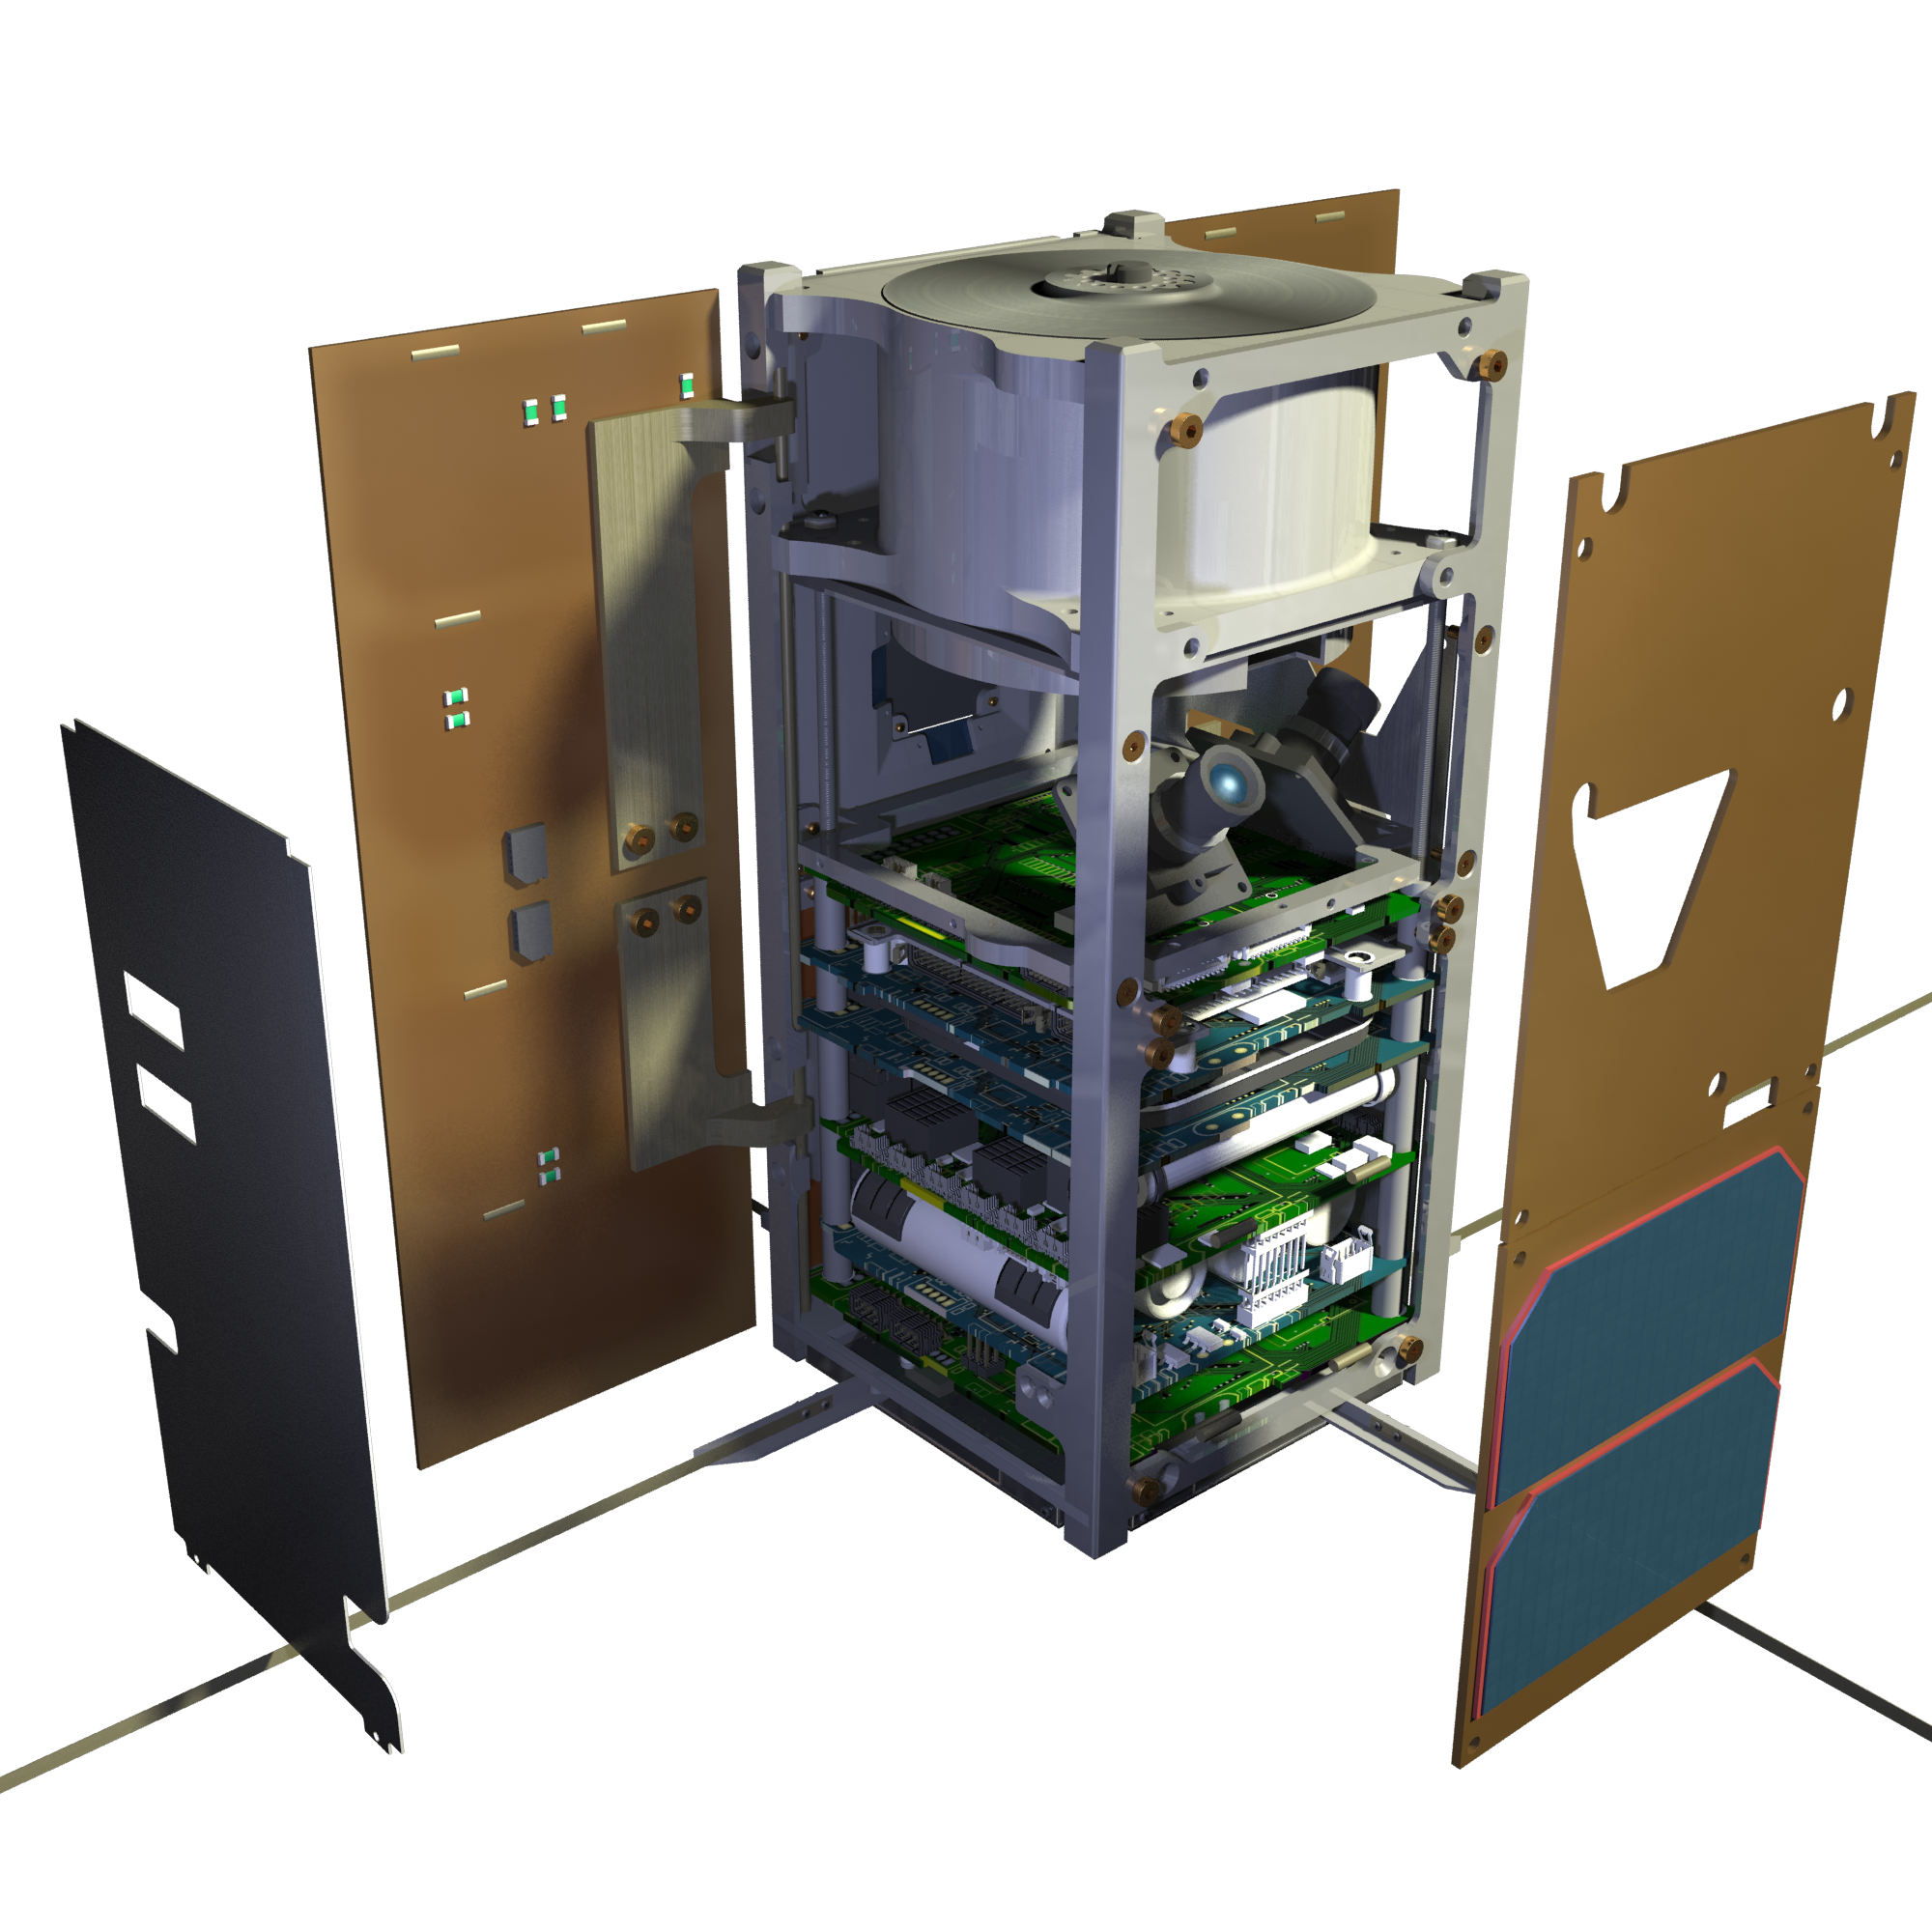
\includegraphics[width=0.65\paperwidth]{img/4/PW-Sat2_render_01.png}
        \caption{PW-Sat2 render. Source: \cite{PW_sat2_photo}}
        \label{PW-Sat_render_01}
    \end{figure}


    \subsection{Primary mission}
    % skopiowane z inż, do przepisania
        The primary mission of PW-Sat2 is to test the deorbit sail. When satellite mission ends, it has to be safely deorbited (or moved to graveyard orbit). Due to new regulations, satellite has to be removed from
        the LEO region no later than 25 years after the end of vehicle operations \cite{Satellite_disposal}. Purpose of deorbit sail is, after satellite operations, to open and increase atmospheric drag, shortening satellite life and cause deorbitation. More information about this experiment can be found in \cite{DDC_article}.

        A render of PW-Sat2 with opened sail is shown in the figure \ref{PW-Sat_render_sail}.

        \begin{figure}[H]
            \centering
            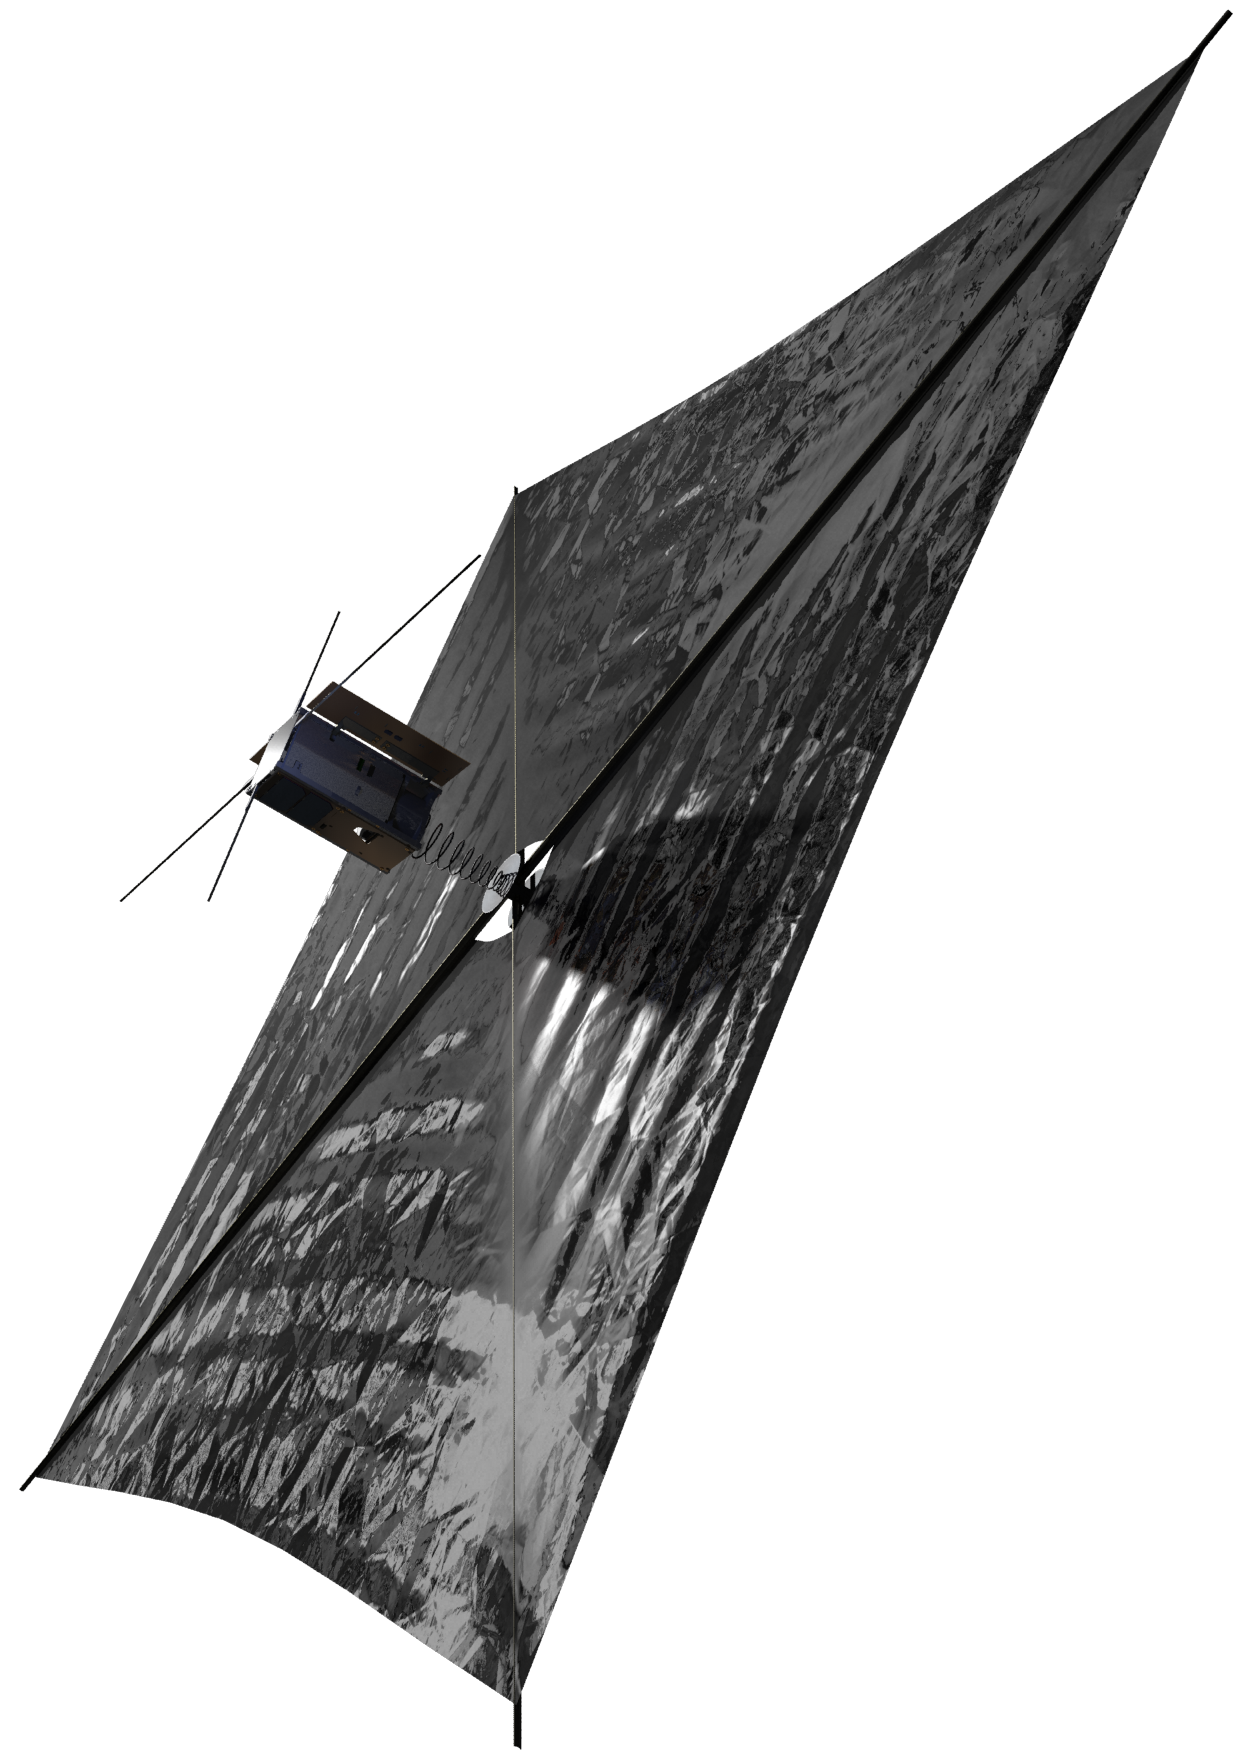
\includegraphics[width=0.38\paperwidth]{img/4/PW-Sat2_render_02.png}
            \caption{PW-Sat2 with opened sail. Source: \cite{PW_sat2_photo}}
            \label{PW-Sat_render_sail}
        \end{figure}

    \subsection{Mission plan and system lifetime}
        PW-Sat2 mission was divided into two phases: normal \& extended mission. Normal phase was planned to take 40 days, after which the deorbitation phase and extended mission begin. Deorbitation can  take up two two years, during which its state along with satellite housekeeping should be monitored.

    \subsection{Orbit}
        PW-Sat2 in planned to be launched to a sun-synchronous circular orbit of attitude \SI{575}{\kilo\meter}, with LTAN of 10:30 \cite{PWSAT_MA_CDR}.



\section{Low Earth Orbit satellite communication review}



\section{Requirements for the system}
\part{System design}

%In this chapter, component selection and design is described.

%During the design process, multiple iteration of component selection, validation and link budget calculation were made, this chapter describes the final result of the link design. 

\chapter{Space segment}
Space segment is a part of the satellite communication system that resides on the satellite itself. It is divided into two main parts: communication subsystem (COMM) and antennas (ANTs) connected with two coaxial cables.

Space segment is critical in system operation and reliability - there is no possibility to carry out any repairs. It is exposed to the space environment - thermal cycling, cosmic radiation and vacuum.

Because of the mentioned requirements it was decided to choose commercially available and flight-proven Cubesat components to increase the reliability of the system.

\section{Frequency band selection}
Data throughput requirements and communication session scheme were described in the \ref{introduction} chapter, but it summarizes to about \SI{1}{\kbps}.

As mentioned in section \ref{aa} the most common radio bands used in Cubesat designs are VHF, UHF and S-band. S-band is usually used when high data rate (~\SI{10}{\Mbps}) are necessary. Typical designs for low-rate data link are full-duplex combo or simplex VHF/UHF radio.

PW-Sat1 (first polish satellite, built on Warsaw University of Technology) - (link)??? used full-duplex VHF-downlink and UHF-uplink radio. During its mission, uplink stability was an issue. The cause was narrowed down to very high level of noise and interference in the UHF band on the orbit, which probably is caused by over-the-horizon radars. Therefore, UHF-uplink was discarded.

Concluding, the selected band for operation were either simplex VHF or VHF-up, UHF-down full-duplex.

\section{Communication subsystem}
Communication subsystem of the satellite is responsible of transmitting and receiving radio signals, modulating/demodulating them and providing data link for the On Board Computer. It has to be compatible with selected mechanical configuration, available data interfaces and the antennas to be installed.

Cubesat standard, with which PW-Sat2 is compliant, defines PC/104 connector, which is the main data bus for all satellite subsystems. Radio should use \iic bus to send and receive data from the on-board computer.

When the subsystem was ordered, the choice of available products was very limited, and the only radio which was compliant with above mentioned requirements was \texttt{ISIS VHF uplink/UHF downlink Full Duplex Transceiver}. Its view and block diagram is shown in the figure \ref{ISIS_TRXvU}

\begin{figure*}
   \centering
\begin{tabular}{cc}
        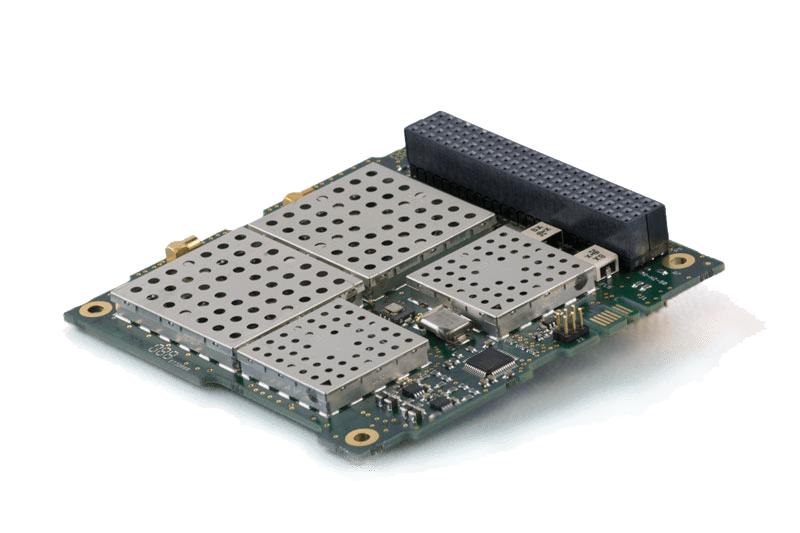
\includegraphics[width=0.4\paperwidth]{img/2/ISIS-radio-UHF-VHF-min.png}
    & 
        %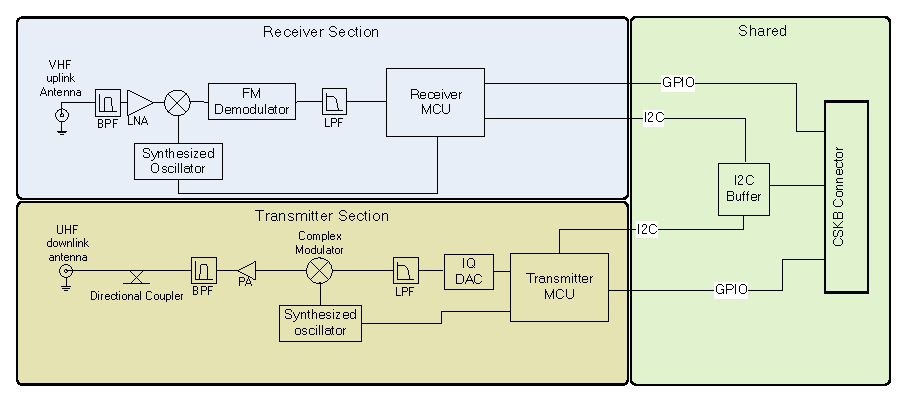
\includegraphics[width=0.3\paperwidth]{img/2/ISIS_TRXvU_block_diagram.eps}
\end{tabular}
\label{ISIS_TRXvU}
\caption{ISIS VHF uplink/UHF downlink Full Duplex Transceiver. Source: \cite{???}}
%%% https://www.isispace.nl/product/isis-uhf-downlink-vhf-uplink-full-duplex-transceiver/
\end{figure*}

Basic characteristics:

\begin{tabular}{c|c}
     \textbf{downlink} & \textbf{uplink} \\ \hline
     \multicolumn{2}{c}{dual-\iic communication standard} \\
     \multicolumn{2}{c}{AX.25 frame format} \\
     \si{430}-\SI{450}{\MHz} frequency range & \si{140}-\SI{150}{\MHz} frequency range \\
     \SI{0.5}{\watt} downlink power & \SI{-98}{\dBm} sensitivity for \si{10^-5}~BER \\
     \si{1.2} - \SI{9.6}{\kilo\bit / \second} bitrate & \SI{1.2}{\kilo\bit / \second} bitrate \\ 
     BPSK modulation with G3RUH scrambling & FM-modulated AFSK \\ 
\end{tabular}



\section{Antennas}
Because of the selected radio system, two antennas has to be installed - one for uplink (VHF) and one for downlink (UHF).

Antennas for this frequencies has to be larger than CubeSat structure - hence  they have to be deployed after release from launcher vehicle. They should be omnidirectional, as PW-Sat2 does not have a pointing possibility and random tumbling is assumed. Typically satellites operate with circular polarization (this is favorable due to satellite rotation), but due to size and weight constraints antenna can have linear polarization.

The most simple antenna for this purpose would be monopole or dipole. Dipole antenna would be more stable in changing objects around - as the PW-Sat will deploy its solar panels and deorbit sail.

Self - made dipole was considered at the design stage, but due to mechanical and time constraints, satellite antenna was decided to be bought. Along with the transceiver, ISIS company does manufacture compatible and tuned antennas for their communication modules. \texttt{CubeSat dipole antenna system} was selected.

This system is deployable by the command from on-board computer. Thermal knife (resistor) is heated up and thermal link is burnt, resulting is antenna deploy by spring action. Antenna is shown in the figure \ref{ISIS_antenna}.

%% TODO: znaleźć zdjęcie złożonej anteny i zmergować
    \begin{figure}[H]
        \centering
        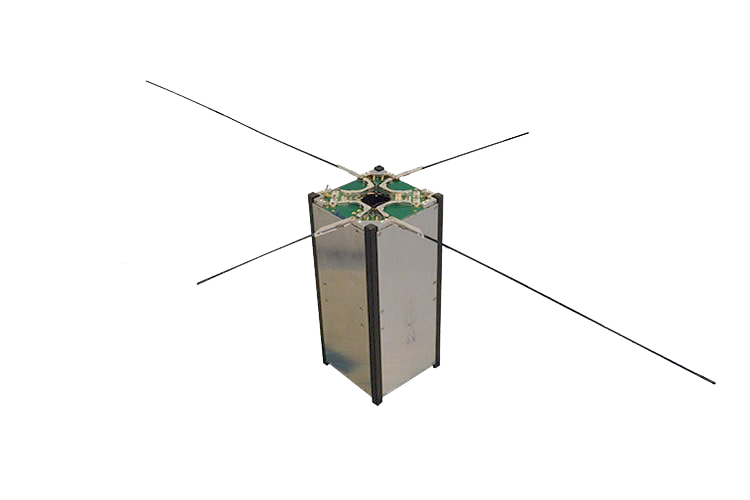
\includegraphics[width=0.8\paperwidth]{img/2/CubeSat-antenna-dipole-configuration.png}
        \caption{ISIS CubeSat dipole antenna system. Source: \cite{???}}
        %%% https://www.isispace.nl/product/dipole-antenna-system/
        \label{ISIS_antenna}
    \end{figure}


\subsection{Deployable elements influence on the antenna pattern}

On-board PW-Sat2 are two main deployables: solar panels and deorbitation sail.

During design stage, influence of the solar panels was discussed with antenna manufacturer - the outcome was to place longed dipoles (VHF) along the solar panels, and shorter ones orthogonally to it, as shown in the figure \ref{???}

% TODO: zdjęcie z otwartymi panelami i antenami

The influence of the deorbit sail was also simulated during Critical Design stage.

Deorbitation sail is made by very thin (\SI{5}{\micro\meter}) mylar foil with aluminium coating. Using % TODO
simulation tool, it was shown that the sail will increase directivity of the cubesat antennas, acting as a reflector.
% TODO: jakieś zdjęcie z symulacji, wynik o ile dB się pogorszyło


\chapter{Communication link parameters}
Selected satellite radio module imposes the modulation and data packets used in the communication. This section briefly describes used modulations, frame formats and implications to the ground segment of the system.

\section{Downlink modulation}
Downlink signal is modulated using Binary Phase Shift Keying (BPSK). The data rate can be changed dynamically by the on-board computer, in range \si{1.2} - \SI{9.6}{\kilo\bit / \second}, allowing to improve the link quality when necessary. Baseband signal is also filtered using Raised Root Cosine filter, to reduce side lobes power. Signal bandwidth varies between \SI{2.4}{\kHz} (for \SI{1.2}{\kbps}) and \SI{19.2}{\kHz} (for \SI{9.6}{\kbps}). 

% TODO: rysunek BPSK

\section{Uplink}
Uplink modulation is two-staged: first, data is modulated using Audio Frequency Shift Keying (chaning 0s and 1s to wave of frequencies, in order, \SI{1200}{\hertz} and \SI{2200}{\hertz}), later to be Frequency Modulated to the RF carrier (with frequency deviation of $\pm\SI{5}{\kilo\hertz}$).

% TODO: schemat modulatora

\section{Frame format}
Physical layer data format is reduced-functionality AX.25 packet \cite{AX25_standard}. Only connectionless transmission mode and UI frames are supported. Packet framing is the same as in SwissCube CubeSat \cite{SwissCube_AX25}.

Basic frame format is shown in the table \ref{AX25_frame}. All the fields except flags are bit-stuffed to ensure that the \textit{Flag} field does not appear in the data: if there are six '1' bits to be send, transmitter inserts '0' bit before the last one. Adressing in this system in inherent, but unused - this is point-to-point connection, therefore adresses are fixed. Frame-Check Sequence is a CRC (CITT standard) of the whole frame (without \textit{Flags}). \textit{Information Field} is variable-length, between \si{4} and \SI{256}{\byte} length is the place for the actual data transmitted by the On-Board Computer.

\begin{table}
\small
\centering
\caption{AX.25 frame format}
\label{AX25_frame}
\arrayrulecolor{black}
\begin{tabular}{l|c|c|c|c|c|c|c|c|} 
\hhline{~|-|----|-|-|-|}
\multirow{2}{*}{}                                                              & \multirow{2}{*}{Flag } & \multicolumn{4}{c|}{AX.25 Transfer Frame Header (128 bits)}                                                                                                                                                                                   & {\cellcolor[rgb]{0.753,0.753,0.753}}                                                                                                                  & \multirow{2}{*}{\begin{tabular}[c]{@{}c@{}}Frame-\\Check\\Sequence\end{tabular}} & \multirow{2}{*}{Flag}  \\ 
\hhline{~|~|-|-|-|-|>{\arrayrulecolor[rgb]{0.753,0.753,0.753}}->{\arrayrulecolor{black}}|~|~|}
                                                                               &                        & \begin{tabular}[c]{@{}c@{}}Destination\\Address\end{tabular} & \begin{tabular}[c]{@{}c@{}}Source\\Address\end{tabular} & \begin{tabular}[c]{@{}c@{}}Control\\Bits\end{tabular} & \begin{tabular}[c]{@{}c@{}}Protocol\\Identifier\end{tabular} & \multirow{-2}{*}{{\cellcolor[rgb]{0.753,0.753,0.753}}\begin{tabular}[c]{@{}>{\cellcolor[rgb]{0.753,0.753,0.753}}c@{}}Information\\Field\end{tabular}} &                                                                                  &                        \\ 
\hline
\multicolumn{1}{|c|}{\begin{tabular}[c]{@{}c@{}}Length\\{[}bits]\end{tabular}} & 8                      & 56                                                           & 56                                                      & 8                                                     & 8                                                            & {\cellcolor[rgb]{0.753,0.753,0.753}}32-2048                                                                                                           & 16                                                                               & 8                      \\ 
\hline
\multicolumn{1}{|c|}{Value}                                                    & 01111110               & PWSAT2-0                                                     & PWSAT2-0                                                & 00000011                                              & 11110000                                                     & {\cellcolor[rgb]{0.753,0.753,0.753}}                                                                                                                  & CRC-CITT                                                                         & 01111110               \\
\hline
\end{tabular}
\end{table}


Additionally, downlink data is scrambled using G3RUH scrambling polynomial to maximize randomness and ensure proper bit synchronization.

%% -------------------------------------------------------------------------------------------

\chapter{Ground station design}
Ground station design should complement the space segment, with large antenna gains and output power to allow the budget link to close.

As the system is full-duplex, both uplink and downlink channels are separate.

\section{Antennas}
Space communication antennas require very large gain due to the distance between the stations. 

Typical design consist of two Yagi-Uda antennas, one for uplink (VHF) and one for downlink (UHF). Their length, therefore directivity was constrained by available space, antenna mast height, antenna rotator strength and positioning accuracy.

PW-Sat2 is transmitting radio signals with linear polarization, nevertheless ground station  polarization should be circular, due to the random tumbling of the satellite. To achieve this, Cross-Yagi antennas were selected, and two linear planes antennas were phased using coaxial cable and symmetrical splitters/combiners. Coaxial cables length was calculated to achieve \SI{90}{\degree} shift between two dipols.

% TODO: schemat anten w GS

Antennas were selected to be the longest possible, limited by mast height. I turned out that they are one of the longest commercially available. 

Antenna characteristics:

\begin{tabular}{c|c}
     \textbf{Downlink} & \textbf{Uplink} \\ \hline
     Tonna & Tonna \\
\end{tabular}


\section{Uplink}
Due to the low sensitivity of the satellite receiver (\SI{-98}{\dBm}) uplink EIRP has to be very large.
\subsection{Transmitter}
Uplink signal is an FM-modulated AFSK, so standard analog audio FM transceiver can be used to generate RF signal. Audio signal can be generated by the Terminal Node Controller or by software running on the PC.

During PW-Sat1 project, the Icom 910H amateur radio transceiver \ref{Icom_910H_ref} was used for both uplink and downlink, therefore it was proposed to use the the same radio.

\begin{figure}[H]
    \centering
    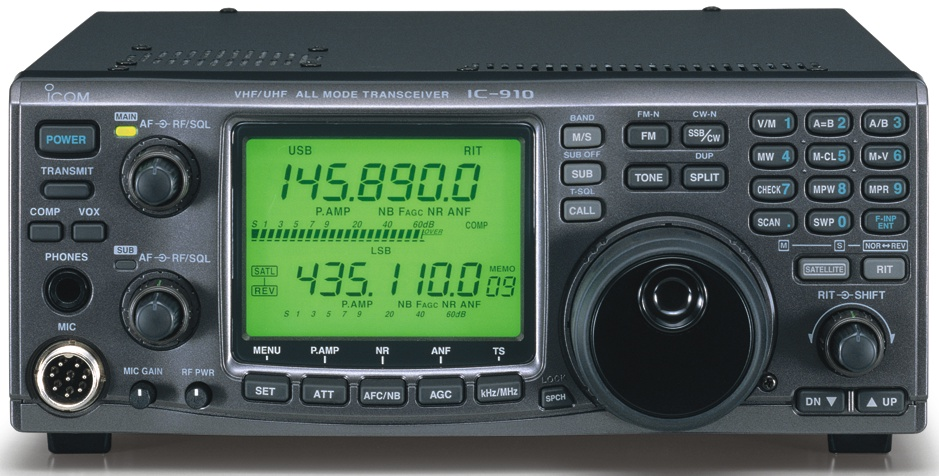
\includegraphics[width=0.6\paperwidth]{img/2/icom910h.jpg}
    \caption{Icom 910H. Source: \cite{ICOM_910H_pic}}
    %%% https://www.isispace.nl/product/dipole-antenna-system/
    \label{Icom_910H_ref}
\end{figure}

Radio VHF FM transmit characteristics:

\begin{tabular}{c|c}
    Frequency & \si{144} - \SI{148}{\MHz} \\
    Frequency stability &  \SI{\pm 3}{\ppm} \\
    Output power & \SI{100}{\watt} \\
    Audio input & analog jack \\
\end{tabular}

This radio is connected to the computer, which controls the audio to transmit and Push-To-Talk (PTT, transmission enable) signal. 

\subsection{Standing Wave Ratio meter}
To check proper antenna connection and ensure long-term monitoring a SWR (Standing Wave Ratio) meter should be installed. This instrument measures ratio of reflected power, thus providing information about antenna impedance matching.

% TODO: zdjęcie/zrzut z kamerki SWR metera



% ------------------------------------------------------------
% ------------------------- DOWNLINK -------------------------
% ------------------------------------------------------------

\section{Downlink}
Receiving Signals from maximal range of about \SI{3000}{\kilo\meter} from a \SI{0.5}{\watt} transmitter requires very high processing gain and low noise factor of the system. Another factor to take into account is Doppler effect, which has to be taken into account. On UHF frequencies, it reaches up to about \SI{15}{\kHz}.

\subsection{Signal front-end processing}
First stage processing has two main purposes - to lower the system noise (amplify the signal) and eliminate intermodulation (filtering).

Downlink system block diagram is shown in the figure \ref{Downln}.

% TODO SCHEMAT DOWNLINKU

Amplifier, installed close to the antenna reduces influence of the long cable to the receiver, reducing total system noise factor. However, strong signals in the proximity of the signal can be intermodulated in the LNA, resulting in variety of issues: from reduced gain to completely distorted signal.

As an amplifier, a high-level Low Noise Amplifier Mini-Circuits PGA-103+ was used, with additional SAW filter to reduce unwanted signals. Schematic and pcb layout of the designed board are shown in the figure \ref{LNA}

% TODO: LNA

Narrowband filter should be installed before the LNA. However, this requires the filter to have the lower loss possible, as the in-band loss in the filter directly affects noise figure of the system. For this purpose, cavity filter was selected. This, reasonably narrow band filter (\SI{1}{\MHz}), has very low insertion loss ($<$\SI{1}{\dB}).

Front-end signal processing was installed as close to the antenna as possible \ref{elka_skrzynka}.

% TODO: elka_skrzynka



To receive BPSK signals, radio amateurs commonly use transceiver with Single SideBand  (SSB) mode. In this mode radio acts as a multi-stage down-converter, allowing to receive baseband with audio card from PC. However, due to audio main purpose, typical radios have a bandpass filters about \SI{3}{\kHz} wide, effectively blocking wider transmissions. Using SSB mode for receiving PW-Sat2 is possible, however only for \SI{1.2}{\kbps} bitrate.

Another options of BPSK receiver is to use integrated transceiver in one chip. This solution is not possible for this system, as no off-the-shelf chips provide AX.25 support.

The proposed receiver so



\chapter{Ground support software}
Due to the Software-Defined Radio based architecture, apart from typical frame processing chain, additional software related to modulation and de-modulation is required.

There are multiple signal processing toolboxes to simplify digital signal processing, such as Matlab/Octave \cite{Matlab}, SciPy \cite{Scipy} and GNUradio \cite{Gnuradio}. GNUradio however, simplifies connecting to physical hardware and programming, by allowing to integrate system in block diagrams.

\section{GNUradio}
% TODO

\section{Data flow chain}
Basic assumption of the data flow was to separate frame building (byte-oriented) from signal processing (sample-oriented). Frame building was written in Python, whereas signal processing was built using GNUradio blocks and self-written custom out-of-tree modules. Communication between the layers was implemented using ZeroMQ asynchronous messaging library. Data flow is shown in the figure \ref{data_flow}.

% TODO: data_flow


\section{Uplink}
Uplink baseband signal (AFSK) has generated, to be later FM-modulated and transmitted using conventional radio.

AFSK signal was generated using software Voltage Controlled Oscillator (VCO), by generating tone (\si{1200} or \SI{2200}{\hertz}) according to the bit value (\si{0} or \si{1}, respectively).  Block diagram of the uplink modulator is shown in the figure \ref{uplink_block}.


\section{Downlink}
The aim of the downlink module is to fully process incoming IQ data from SDR to baseband data (frames).




\section{Satellite operation}


\part{Component and system verification}

% In this chapter, whole system design verification is described. 


\chapter{Space segment verification}

Satellite communication subsystem have to be thoroughly tested on the ground, as once sent nothing can be changed or fixed. High quality measurements are required to verify functionality of the system in the changing environment.

\section{Flatsat}

Most of the tests were performed on Flatsat (an abbreviation from Flat Satellite), an electronic test bench, which consist of mix of flight models, engineering models of the instruments and Electrical Ground Support Equipment (EGSE). EGSE are the test instruments and/or mocks (fake) instruments, which allow testing without the need for actual hardware.

PW-Sat2 Flatsat was integrated in Space Research Centre in Warsaw. Flatsat is shown in the figure \ref{TODO}.

\subsection{Flatsat Ground Station mock}
To perform the communication tests a Ground Station mock was created of flatsat. It was built using to Software-Defined Radios: one, as downlink receiver, same as to be installed in the Ground Station (Funcube Pro+), and the second (PlutoSDR) to generate uplink signals. Use of SDR instead of analogue radio transceiver greatly simplified the tests performed. Ground station mock is shown in the figure \ref{TODO}. 


\section{Transceiver measurement}
Transceiver was tested separately for its uplink and downlink capabilities. Tests are critical to make sure that radio parameters are maintained in the system, and to verify manufacturers' data.

\subsection{Uplink}
The most important parameter of the radio receiver is the sensitivity. Blocking immunity (intermodulation), is not critical, as the system is remote from most of the external strong radio signals.

\subsubsection{Sensitivity}
Sensitivity was measured by the setup shown in the figure \ref{TODO}. Test procedure:
\begin{itemize}
    \item measuring output power of PlutoSDR using spectrum analyzer with wide RBW filter (\SI{1}{\MHz})
    \item increasing attenuation up to the point when PER is noticeable (\SI{1}{\percent})
    \item calculating signal input power
\end{itemize}

The result of this test was the sensitivity of TODO.

\subsubsection{Doppler}
Doppler effect is caused when fast-moving object is emitting/receiving radio waves. For uplink frequency (VHF band) Doppler effect influence can shift frequency up to about \SI{5}{\kHz}. The receiver bandwidth should be measured to estimate allowable frequency inaccuracies.

Test setup is the same as in previous setup, shown in the figure \ref{TODO}. During the test the PER was measured for a range of frequency shift from center. The result is shown in the chart \ref{TODO}.

\section{Satellite antennas}
After deployment on the orbit, antennas have to deploy. During the test campaign antenna deployment procedure was executed three times. Deployed antennas are shown in the figure \ref{TODO}.

Reflected power from antenna is measured by the radio module during radio frame transmission. Correct antenna deployment can be assured by using the telemetry and comparing the reflected power with measured during the ground test campain. 
Reflected and forward power chart captured during second antenna opening are shown in the figure \ref{TODO}. 



\subsection{Downlink}
Downlink parameters of the radio module were also measured. An important parameter is the output power and the spectrum of the signal.

\subsubsection{Output power}
Output power was measured using spectrum analyser with wide resolution bandswidth (\SI{1}{\MHz}). Output power was measured to be \SI{27}{\dBm}. TODO

\subsubsection{Spectrum}


% ------------------------------------------------------
% ------------------------------------------------------
% ------------------------------------------------------

\chapter{Ground segment verification}
The design of the ground segment had to be also verified to make sure that the assumed requirements were met.

\section{Antenna measurement}
After the assembly, antennas should be measured to make sure of the correct assembly. The simplest method is to measure the impedance of the antennas.

Each antenna consist of two dipoles (with vertical and horizontal polarizations) phased with a combiner. Measurements of the dipoles and the phased antenna were performed, and the result is shown in the table \ref{TODO}.


\section{Uplink}
As the uplink was built using conventional HAM radio transceiver, only the modulation and output power should be measured. As the physical layer is the typical FM-modulated AFSK and frame protocol is typical AX.25 there is a lot of free software to verify the correctness of the frame and modulation.

\subsection{Output power}
The power of the power amplifier (built in the transceiver) was measured using an SWR \& Power Meter TODO, and by connecting radio output to the antenna. The measured output and SWR was equal to TODO. Those parameters are continuously monitored during the mission to monitor the cables and radio health.

\subsection{Spectrum \& Watchdogs}
The spectrum and output modulation correctness in constantly monitored using so-called watchdogs built using another Software Defined Radios (PlutoSDR, RTL-SDR) placed in the proximity of the main antennas.
By demodulating uplink signal and comparing it in the real time with transmitted frames the correctness of the transmission is guaranteed. Watchdog flowchart and graphical view are shown in the figure \ref{TODO}.



\section{Downlink}
Downlink radio flow is shown in the figure \ref{TODO}. Radio chain verification was performed step-by-step, starting from Low-Noise Amplifier and ending on receiver sensitivity.

\subsection{Band pass filter}
Cavity filter was tuned to the required frequency to minimize insertion loss and bandwidth. Signal bandwidth is very narrow compared to the filter frequency range.
The insertion loss and band pass range was measured using Network Analyser. S-parameters are shown in the figure \ref{TODO} and the filter parameters are summarised in the table \ref{TODO}.


\subsection{Low Noise Amplifier}
Designed Low Noise Amplifier is shown in the figure \ref{TODO}. Its S-parameters were tested using Rohde\& Schwarz ZVL. Results are shown in the figure \ref{TODO}. Gain and frequency were as expected and are shown in the table \ref{TODO}.



\subsection{Receiver measurements}
Receiver block diagram is shown in the figure \ref{TODO}. The most important blocks for testing are the demodulator itself and frequency correction block.

\subsubsection{Frequency correction block}
Frequency correction block was tested using already flying satellites, verifying stability of frequency after correction.


\subsubsection{Demodulator}
The demodulator was designed for two major cases:
\begin{itemize}
    \item wide bandwidth and large frequency correction (when orbit Keppler data is not well-known, resulting in unpredicted Doppler shift),
    \item wide bandwidth and no frequency correction (when orbit Keppler data is well-known resulting in negligible frequency inaccuracies).
\end{itemize}

Depending on the case, different parameters of the Costa's loop were determined. Both test-cases were implemented and the sensitivity and maximum frequency shift were determined.

The test setup for measuring demodulator is shown in the figure \ref{TODO}, and consist of:
\begin{itemize}
    \item PlutoSDR - transmitter of the frames with regulated center frequency and output power,
    \item attenuators
    \item Funcube Pro+ SDR - receiver used in the ground station
\end{itemize}

Frames to be transmitted were recorded with Software-Defined Radio during flatsat campaign and replayed during sensitivity tests. This ensures that all the important inadequacies transmitted by the radio transmitter were also taken into account.
With the test setup, sensitivity was automatically measured by varying output power of the transmitter (in \SI{0.25}{\dB} steps) and PER was recorded for each point. During the process, different parameters of the demodulator were tuned to increase the sensitivity. Final results are shown in the table \ref{TODO} and figures \ref{TODO} - \ref{TODO}.


\part{Mission results}
At $3^{rd}$ of December 2018, PW-Sat2 was launched on \SI{590}{\kilo\meter} orbit on-board Falcon9 rocket from SpaceX company. 

\section{Lanuch and Early Operations Phase}
During first hours after launch, PW-Sat2 was inside the container, completery turned off by the kill-switch. 4 hours after the launch, it was deployed and turned on automatically. On-Board software, after silent period of \SI{30}{\minute} performed antenna deployment procedure and started transmitting beacon data every \SI{60}{\second}.

%TODO http://k4kdr.github.io/
Beacon data (consisting of satellite telemetry) was received first by Scott Chapman (K4KDR) from United States of America at 6:10 am the day after launch. Later, during the first couple of days of orbital operations the Bus and Payload commissionings were performed.

During first sessions, satellite was transmitting with \SI{1200}{\bps} downlink speed, providing reliable radio link. PW-Sat2 took first polish satellite photograph \ref{TODO} at \si{5^{th}} of December 2018. It was taken by a part of camera built-in tests and downloaded on request from ground.


\section{Doppler correction}
During the launch, \si{64} satellites were launched together and were separated from the upper stage of the rocket by spring actions. At first, they were flying together and with the time, they were further apart from each other. Figure \ref{TODO} show the on-orbit position of the satellites on \si{25^{th}} day after the launch. Doppler effect estimation was performed during every pass, with increased accuracy. Typical method for selecting an satellite object from a set of different ones is done by applying Doppler correction to the received signal spectrum, for every object in the field of view, and later choosing the most suited one. 

Signal before and after Doppler correction is shown in the figure \ref{Doppler_correction_gqrx}.

\begin{figure}[H]
    \centering
    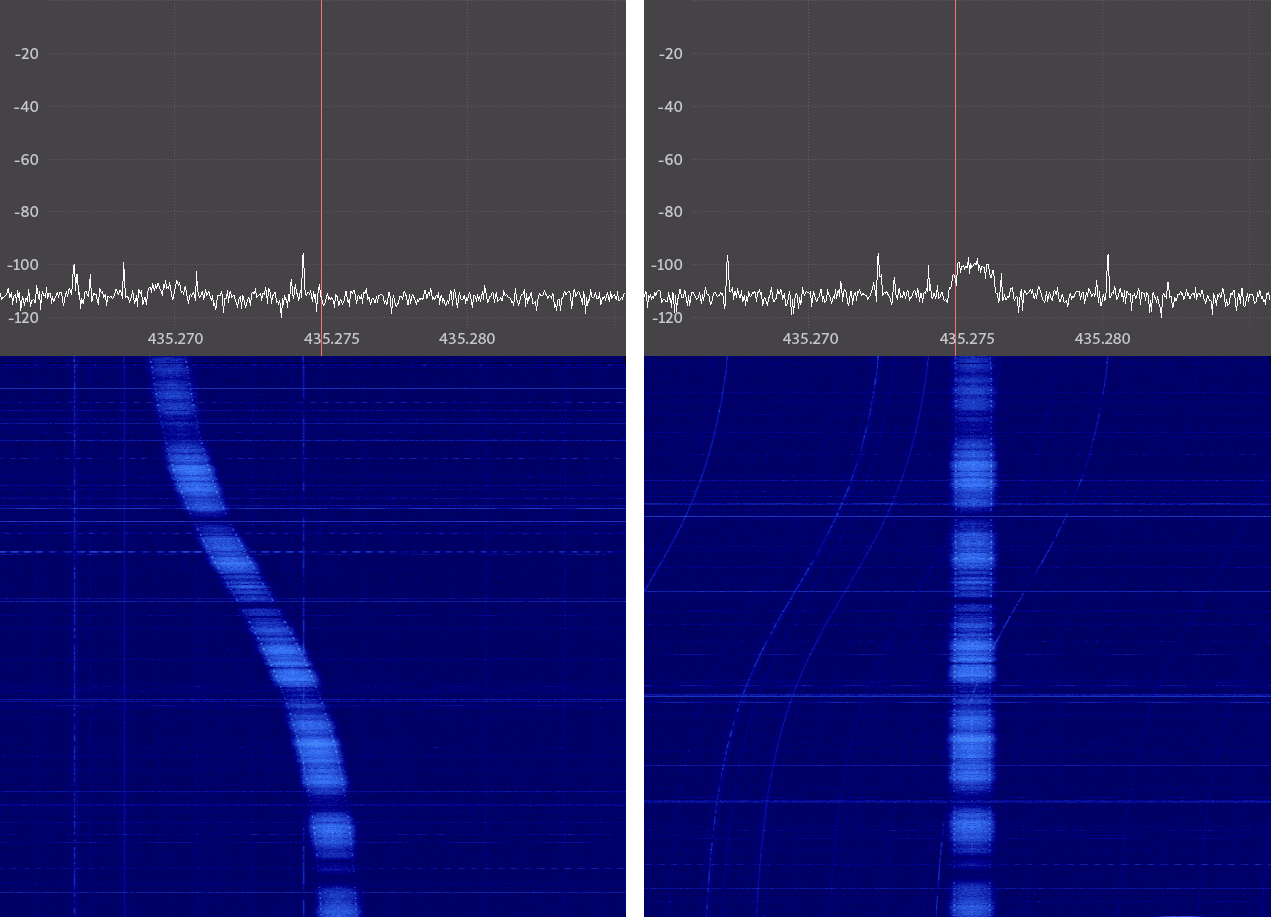
\includegraphics[width=0.65\paperwidth]{img/4/doppler_correction.png}
    \caption{Doppler correction.}
    \label{Doppler_correction_gqrx}
\end{figure}

\section{Link budget estimation}


\section{Main mission results}






\appendix
\printbibliography

\end{document}
